
\chapter{Modelo Dinâmico}
\label{sec-modelo-dinamico}

O modelo dinâmico visa capturar o comportamento dinâmico do sistema. A seguir, são
apresentados os diagramas de estados e o diagrama de atividades elaborados no contexto deste
projeto.


\section{Diagramas de Estados}


A Figura~\ref{figura-estado-depoimento} apresenta o diagrama de estados da classe Depoimento do subsistema Public.

\begin{figure}[h]
  \centering
  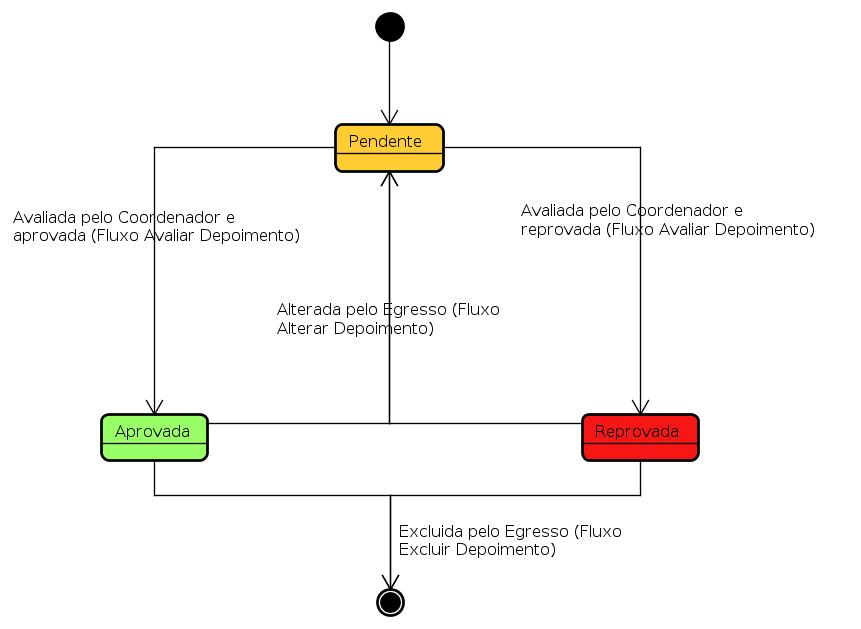
\includegraphics[scale=0.45]{figuras/estado-depoimento.jpg}
  \caption{Diagrama de Estados da Classe Depoimento.}
  \label{figura-estado-depoimento}
\end{figure}
